%\chapter{超音波擔傷試験の数値シミュレーション法}
\section{問題設定}
図\ref{fig:fig2_0}に,本研究で想定するT継手における超音探傷の状況設定を示す.
継手は,水平部材に対して直角に近い角度で板材が溶接されているとし,以下では便宜上,水平部材をウェブ,鉛直向きの板材をフランジと呼ぶ.
溶接部の詳細はこの図には示していないが,片側(右側)からの隅肉溶接が行われているとし,
継手右側を外側,左側を内側と称する.内,外の呼び方は,Uリブ断面にこの状況を当てはめたときの区分である。
なお,次章で示す数値シミュレーション結果では,比較のために溶接部の余盛りを無視し,ウェブとフランジが溶接金属が追加されることなくそのまま結合されたモデルと,厚みが一定の平板に対する結果を示す.
き裂は,継手内側の角部から発生してフランジ面に対して鉛直に伸びるものを考える.
現実には,継手に生じる応力場によってき裂の進展方向が変化するため,起点が同じでも溶接金属内やウェブ側にき裂が伸びるケースもある.その場合,き裂評価にはウェブ側からの探傷が必要で,超音波の送受信や伝播状況が図のものと大きくことなり,別途,考察の対象とする必要があるので本研究では扱わない.
超音波の送受信は,継手外側のフランジ上面でのみ実施可能とする.従って,送信,受信方向はき裂に対して強く制約され,検査に利用できる超音波エコーはき裂からの後方散乱波だけとなる.もし,送受信子をき裂を挟むように,継手左右に置くことがことができるならば,よく知られたTOFD法(time-of-flight diffraction)が利用できる.
ここでは,TOFDが適用できない、より困難な状況を想定した問題として片側からの探傷を扱う.
%--------------------
\begin{figure}[h]
	\begin{center}
	\includegraphics[width=0.8\linewidth]{Figs/setup.eps} 
	\end{center}
	\caption{
		(a) T継手をもつ橋梁構造部分の例(鋼床版Uリブ取付位置の溶接部).
		(b) T継手における片側からの超音波探傷試験.
	} 
	\label{fig:fig2_0}
\end{figure}
%--------------------
超音波の送信は,鋼橋の超音波探傷で通常用いられる圧電探触子によって,フランジ上面から行う.ただし,数値シミュレーションでは,圧電素子を直接モデル化することを避け,既知の鉛直力分布で与える.
この方法では,鉛直力の時間変化に位相差がない場合,探触子からの垂直入射を模擬できる.
一方,空間的に直線的な位相差をつけた鉛直力を与えれば,斜角入射を模擬できる.
受信は無指向性の点レシーバにより,継手外側の任意の範囲で行うことができるとする.
これは,波長に対して十分に小さいアレイ探触子での受信を想定したものである.
実際の探傷には,必ずしもアレイセンサーを用いるわけでは無いが,アレイセンサーで受信した波形群を適切な遅延時間を設けて重ね合わせることで,斜角探触子による受信も模擬できる.この意味で,今回の設定は,一般のセンサー
による受信波形を模擬できるという意味で包括的なものと言える.
\section{波動伝播問題の定式化}
鋼橋の超音波探傷試験に用いる超音波の周波数帯はおよそ2MHzから5MHzで,その振幅は数十nm程度と非常に小さい.そのため,超音波伝搬は微小変形問題で,媒体は線形弾性体とみなした解析を行うことができる.
このとき,弾性波動問題の支配方程式は,応力$\sigma_{ij}$, 速度$v_i$,
質量密度$\rho$を用いて
\begin{equation}
	\sigma_{ji,j}+f_i=\rho \dot{v}_i,
	\label{eqn:}
\end{equation}
で与えられる.ただし,$(,)$は空間の$\dot{()}$は時間に関する微分
\begin{equation}
	(\cdot)_{,i}=\frac{\partial (\cdot)}{\partial x_i}, \ \ 
	\dot{(\cdot)}=\frac{\partial (\cdot)}{\partial x_i}, \ \ 
	\label{eqn:}
\end{equation}
をそれぞれ表す.ここでは2次元問題を考えるため,インデックス$i,j$は1または2をとり,上の式では総和規約を適用して表記している.速度$v_i$は変位$u_i$の時間微分であり,ひずみテンソル$\varepsilon_{ij}$は,
変位を使って
\begin{equation}
	\varepsilon_{ij}=\frac{1}{2}(u_{i,j}+u_{j,i})
	\label{eqn:}
\end{equation}
で与えられる.応力テンソルは弾性係数テンソル$C_{ijkl}$として
を用いて次のように表される.
\begin{equation}
	\varepsilon_{ij}=C_{ijkl}\varepsilon_{kl}
	\label{eqn:}
\end{equation}
ただしここでは媒体を等方性体とみなし,
\begin{equation}
	C_{ijkl}=\lambda \delta_{ij}\delta_{kl} +2\mu \delta_{ik}\delta_{jl}
	\label{eqn:}
\end{equation}
とする.ここに,$\lambda, \mu$はラメ定数を表す.ラメ定数と密度より,
縦波と横波の位相速度は,順に
\begin{equation}
	c_{P}=\sqrt{\frac{\lambda + 2\mu}{\rho}}
	, \ \ 
	c_{S}=\sqrt{\frac{\mu}{\rho}}
	\label{eqn:}
\end{equation}
と与えられる.工学でしばしば用いられるヤング率$E$,ポアソン比$\nu$,せん断剛性$G$を
との関係は次のようになる.
\begin{equation}
	E=\frac{\mu(3\lambda + 2\mu )}{\lambda+\mu}, \ \ 
	G=\mu,\ \
	\nu =\frac{\lambda}{2(\lambda+\mu)} 
	\label{eqn:}
\end{equation}
以上の式を与えられた初期条件,境界条件の元で解くことで,超音波の伝播シミュレーションを行う.
\section{数値解析法(FDTD法)}
前節で示した方程式に離散化に,FDTD(Finite Difference Time-Domain)法を用いる.
ここで,時間ステップ長を$\Delta t$, スタガード格子の$x_i$軸方向の間隔を
$\Delta x_i,(i=1,2)$とし,その間隔は一定とする.
この間隔で時空間内に配置された差分格子における関数$f(\fat{x},t)$の値を$f^k_{i,j}$と書くことにする.ただし,$k$は時間ステップを,$i,\, j$は$x_1$および$x_2$方向の格子位置を表す番号を意味する.このとき,中央差分で時間微分を近似すれば,
\begin{equation}
	\dot{f}^{k+\frac{1}{2}} \approx \frac{ (f)^{k+1}-(f)^k}{\Delta t}
	\label{eqn:dfdt}
\end{equation}
となり,後に示すように,整数時間ステップ$k$で$f^k$を,半整数時間ステップ$t^{k+\frac{1}{2}}$において$\dot f$を,初期値$f^0, \dot f^{\frac{1}{2}}$から交互に求める蛙飛び差分(リープフロッグ)法による差分方程式が得られる.一方,空間微分$\nabla f$は
\begin{eqnarray}
	\left( \frac{\partial f}{\partial x_1}\right)
	_{i+\frac{1}{2}, \, j+\frac{1}{2}}
	& \approx &
		\frac{\left(f\right)_{i+1,j+\frac{1}{2}} -\left(f\right)_{i,\, j+\frac{1}{2}}}
		{\Delta x_1}
	\label{eqn:dfdx1}
	\\
	\left( \frac{\partial f}{\partial x_2}\right)
	_{i+\frac{1}{2}, \, j+\frac{1}{2}}
	& \approx &
	\frac{\left(f\right)_{i+\frac{1}{2},j+1} -\left(f\right)_{i+\frac{1}{2},\, j}}{\Delta x_2}
	\label{eqn:dfdx2}
\end{eqnarray}
と近似する.このような差分化を行うためには,関数$f$とその勾配$\nabla f$の計算格子がスタガード格子を形成するように配置しておけばよい.
%%%%%%%% FIGURE 2 %%%%%%%%%
%	FD GRID
\begin{figure}
     \begin{center}
     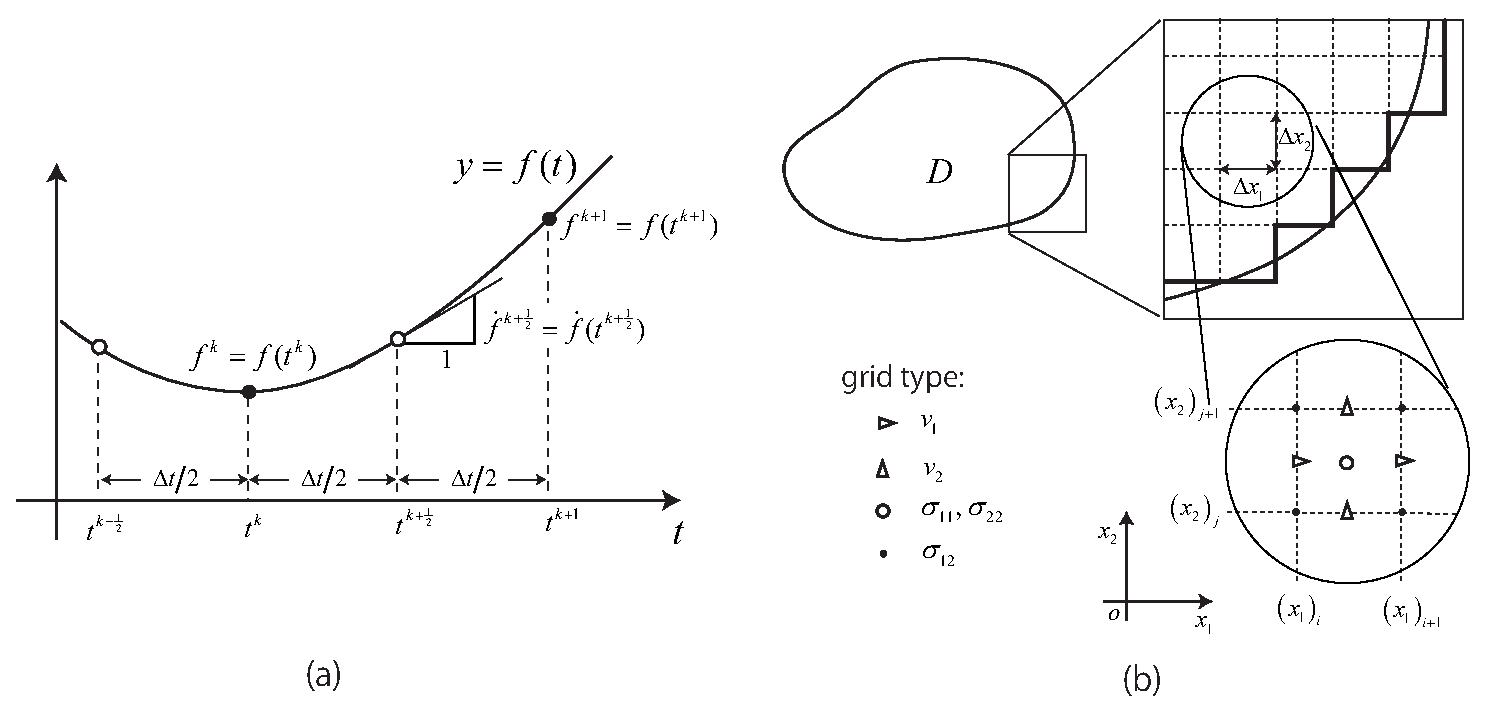
\includegraphics[width=1.0\linewidth]{Figs/FDgrid.eps}
     \end{center}
     \caption{ (a) リープフロッグ法に対する時間方向への差分格子配置.
	 (b) 空間の離散化を行うためのスタガード格子配置. 
	}
     \label{fig:FDgrids}
\end{figure}
%%%%%%%%%%%%%%%%%%%%%%%%%%%
スタガード格子は図\ref{fig:FDgrids}に示したような,直応力の計算格子を中心にした$\Delta x_1 \times \Delta x_2$の矩形領域の頂点にせん断応力の,辺上に速度の計算格子を配置したセルを基本単位とする格子配置をとる.これらの格子点における関数値を用いて, 動弾性問題の支配方程式を差分近似すれば,以下のような結果が得られる.
\begin{equation}
	\rho \frac{(v_1)_{i,j+\frac{1}{2}}^{k+1}-(v_1)^k_{i,j+\frac{1}{2}}}{\Delta t}
	=
	\frac{ 
		(\sigma_{11})^{k+\frac{1}{2}}_{i+\frac{1}{2},j+\frac{1}{2}}
		-(\sigma_{11})^{k+\frac{1}{2}}_{i-\frac{1}{2},j+\frac{1}{2}} 
	}
	{\Delta x_1}
	+
	\frac{(\sigma_{12})^{k+\frac{1}{2}}_{i,j+1}-(\sigma_{12})^{k+\frac{1}{2}}_{i,j}}{\Delta x_2}
	\label{eqn:fdtd_v1}
\end{equation}
\begin{equation}
	\rho \frac{(v_2)_{i+\frac{1}{2},j}^{k+1}-(v_2)^k_{i+\frac{1}{2},j}}{\Delta t}
	=
	\frac{(\sigma_{12})^{k+\frac{1}{2}}_{i+1,j}-(\sigma_{12})^{k+\frac{1}{2}}_{i,j}}{\Delta x_1}
	+
	\frac{ 
		(\sigma_{22})^{k+\frac{1}{2}}_{i+\frac{1}{2},j+\frac{1}{2}}
		-(\sigma_{22})^{k+\frac{1}{2}}_{i+\frac{1}{2},j-\frac{1}{2}} 
	}
	{\Delta x_2}
	\label{eqn:fdtd_v2}
\end{equation}
\begin{equation}
	\frac{
		 (\sigma_{11})^{k+\frac{1}{2}}_{i+\frac{1}{2},j+\frac{1}{2}}
		-
		 (\sigma_{11})^{k-\frac{1}{2}}_{i+\frac{1}{2},j+\frac{1}{2}}
	}
	{\Delta t}
	=
	\left( \lambda+2\mu \right)
	\frac{
		(v_1)^{k}_{i+1,j+\frac{1}{2}} - (v_1)^{k}_{i,j+\frac{1}{2}} 
	}
	{\Delta x_1}
	+
	\lambda
	\frac{
		(v_2)^{k}_{i+\frac{1}{2}, j+1} - (v_2)^{k}_{i+\frac{1}{2},j} 
	}
	{\Delta x_2}
	\label{eqn:fdtd_s11}
\end{equation}
\begin{equation}
	\frac{
		 (\sigma_{22})^{k+\frac{1}{2}}_{i+\frac{1}{2},j+\frac{1}{2}}
		-
		 (\sigma_{22})^{k-\frac{1}{2}}_{i+\frac{1}{2},j+\frac{1}{2}}
	}
	{\Delta t}
	=
	\lambda
	\frac{
		(v_1)^{k}_{i+1,j+\frac{1}{2}} - (v_1)^{k}_{i,j+\frac{1}{2}} 
	}
	{\Delta x_1}
	+
	\left( \lambda+2\mu \right)
	\frac{
		(v_2)^{k}_{i+\frac{1}{2}, j+1} - (v_2)^{k}_{i+\frac{1}{2},j} 
	}
	{\Delta x_2}
	\label{eqn:fdtd_s22}
\end{equation}
\begin{equation}
	\frac{
		 (\sigma_{12})^{k+\frac{1}{2}}_{i,j}
		-
		 (\sigma_{12})^{k-\frac{1}{2}}_{i,j}
	}
	{\Delta t}
	=
	\mu \left(
		\frac{
			(v_2)^{k}_{i+\frac{1}{2},j}
			-
			(v_2)^{k}_{i-\frac{1}{2},j}
		}
		{\Delta x_1}
		+
		\frac{
			(v_1)^{k}_{i,j+\frac{1}{2}}
			-
			(v_1)^{k}_{i,j-\frac{1}{2}}
		}
		{\Delta x_2}
	\right)	
	\label{eqn:fdtd_s12}
\end{equation}
以上の式のうち,式(\ref{eqn:fdtd_v1})から(\ref{eqn:fdtd_v2})を,$(v_1)^{k+1}_{i,j+\frac{1}{2}}$や$(v_2)^{k+1}_{i+\frac{1}{2},j}$について解けば, 速度と応力を交替に求める蛙飛び差分スキームによる差分公式が得られる.なお,以上の結果は領域内部にある計算格子において適用可能なものであるため,境界上のグリッドについては,指定された境界条件を反映した差分方程式を用いる必要がある.ここでは,トラクションが与えられた境界における境界条件の与え方について述べる.いま,計算領域を差分セルの集合で近似することを考えると,境界上に配置される可能性のある計算格子は$v_1, v_2$および$\sigma_{12}$である.このうち$\sigma_{12}$については,与えらえた境界値をそのまま代入すればよい.一方,速度$v_1, v_2$については,単位セルサイズが半分になったものと考え,運動方程式を有限体積法の考え方に従って離散化すれば,次のような差分方程式が得られる.
\begin{equation}
	\rho \frac{(v_1)_{i,j+\frac{1}{2}}^{k+1}-(v_1)^k_{i,j+\frac{1}{2}}}{\Delta t}
	=
	\alpha
	\frac{ 
		(\bar\sigma_{11})^{k+\frac{1}{2}}_{i,j+\frac{1}{2}}
		-(\sigma_{11})^{k+\frac{1}{2}}_{i-\frac{\alpha}{2},j+\frac{1}{2}} 
	}
	{\Delta x_1/2}
	+
	\frac{(\bar \sigma_{12})^{k+\frac{1}{2}}_{i,j+1}-(\bar \sigma_{12})^{k+\frac{1}{2}}_{i,j}}{\Delta x_2}
	\label{eqn:fdtd_v1_bnd}
\end{equation}
\begin{equation}
	\rho \frac{(v_2)_{i+\frac{1}{2},j}^{k+1}-(v_2)^k_{i+\frac{1}{2},j}}{\Delta t}
	=
	\frac{(\bar\sigma_{12})^{k+\frac{1}{2}}_{i+1,j}-(\bar\sigma_{12})^{k+\frac{1}{2}}_{i,j}}{\Delta x_1}
	+
	\beta
	\frac{ 
		(\bar \sigma_{22})^{k+\frac{1}{2}}_{i+\frac{1}{2},j}
		-(\sigma_{22})^{k+\frac{1}{2}}_{i+\frac{1}{2},j-\frac{\beta}{2}} 
	}
	{\Delta x_2/2}
	\label{eqn:fdtd_v2_bnd}
\end{equation}
ただし,$\bar{(\cdot)}$は既知の境界値であることを意味し,式(\ref{eqn:fdtd_v1_bnd})と(\ref{eqn:fdtd_v2_bnd})に含まれるパラメータ$\alpha$および$\beta$は,
 \begin{equation}
	\alpha=(n_1)_{i,j+\frac{1}{2}}, \ \ \beta=(n_2)_{i+\frac{1}{2},\, j},
	\label{eqn:def_ab}
\end{equation}
で,外向き法線ベクトル$\fat{n}=(n_1,\, n_2)$の方向により1または-1をとる.以上を用いて,超音波伝播解析を2次元問題として行った結果を次章、次々章に示す.
%%%%%%%%%%
